\documentclass[]{article}

\usepackage{todonotes}
\usepackage{graphicx}
\usepackage{float}

%opening
\title{Remote Batteryless Internet-of-Things Sensor Testbed}
\author{B.T. Blokland}

\begin{document}

\maketitle

\section{Introduction}

The Internet-of-Things (IoT) is a promising vision which enables trillions of sensor devices to be connected. A common bottleneck for such devices is the energy supply. Batteries are large, expensive, heavy and wear out after several years.

A more sustainable solution than batteries, is energy harvesting where a device collects it's energy from the environment i.e. solar, radio frequency (RF), thermal or kinetic energy.

However, developing software for such devices comes with a challenge. Environmental energy can be scarce, causing frequent power failures. This contrasts with the standard assumption that programs run continuously throughout execution. The programmer has to take care of this intermittent behavior by i.e. storing data to non-volatile memory at certain intervals. The available energy tends to be random, making it difficult to predict how long a program can execute before the next power failure. 

It is hard to conduct repeatable tests due to the random nature of the energy source. While comparing two algorithms, it is impossible to conclude that one algorithm outperforms the other without knowing how much the difference in available energy contributed to the result.

The goal of this thesis is to make a testbed that counters this issue, by using Ekho \cite{ekho}. This an emulator capable of accurately recreating, repeatable harvesting conditions in a lab. The testbed will be made remotely accessible to reduce the effort of setting up such an environment and accelerating development in this field of study.
 
\section{Related Work}

For batteryless devices there are no publicly available testbeds. This paper \cite{request} enlists properties and features that any batteryless devices testbed should have, calling for more coordinated action in this domain research. It also presents a minimal implementation of such a testbed.

There has been extensive research into the field of Wireless Sensor Networks (WSN) testbeds, which have closely related features. Besides these testbeds, there are several tools which help in developing applications for battery less devices. These will be discussed as well.

\subsection{Wireless Sensor Networks}
%todo{Paraphrase this section, taken from https://www.iotbench.ethz.ch/}

\subsubsection{FIT IoT-LAB}
FIT IoT-LAB \cite{FIT-IoT} provides a very large scale infrastructure facility suitable for testing small wireless sensor devices and heterogeneous communicating objects.

IoT-LAB features over 2000 wireless sensor nodes spread across six different sites in France.  Nodes are either fixed or mobile and can be allocated in various topologies throughout all sites.  A variety of wireless sensors are available, with different processor architectures (MSP430, STM32 and Cortex-A8) and different wireless chips (802.15.4 PHY @ 800 MHz or 2.4 GHz).  In addition, “open nodes” can receive custom wireless sensors for inclusion in IoT-LAB testbed.

\subsubsection{Flocklab}

Flocklab \cite{flocklab} is a wireless sensor network (WSN) testbed, developed and run by the ​Computer Engineering and Networks Laboratory at the ​Swiss Federal Institute of Technology Zurich (ETH Zurich) in Switzerland. FlockLab's key features include:
\begin{itemize}
	\item FlockLab's observer based testbed architecture which provides services for detailed testing of sensor nodes:
	\item Time accurate pin tracing
	\item Time accurate pin actuation
	\item Power measurements
	\item Serial interface logging and writing
	\item Voltage control to simulate e.g. battery depletion
\end{itemize}

\subsubsection{Indriya2}

Indriya2 \cite{indriya2} is a three-dimensional wireless sensor network deployed across three floors of the School of Computing , at the National University of Singapore (NUS). The Testbed facilitates research in sensor network programming environments, communication protocols, system design, and applications. It provides a public, permanent framework for development and testing of sensor network protocols and applications. Users can interact with the Testbed through an intuitive web-based interface designed based on Harvard's Motelab's interface. Registered users can upload executables, associate those executables with motes to create a job, and schedule the job to be run on Testbed. During the job execution, all messages and other data are logged to a database which is presented to the user upon job completion and then can be used for processing and visualization. 

\subsection{Development tools for batteryless devices}

\subsubsection{Ekho}

To counter the issue of randomness in a energy harvesting power source, Ekho \cite{ekho} has been developed. This an emulator capable of accurately recreating harvesting conditions in a lab. It reproduces the I-V characteristics of energy harvesting sources, allowing developers to choose from a library of energy traces recorded with various sources and environmental conditions.

\subsubsection{Flicker}
%todo{Paraphrase this section}
Flicker \cite{flicker} is a platform for quickly prototyping batteryless embedded sensors. Flicker is an extensible, modular, “plug and play” architecture that supports RFID, solar, and kinetic energy harvesting; passive and active wireless communication; and a wide range of sensors through common peripheral and harvester interconnects. Flicker supports recent advances in failure-tolerant timekeeping, testing, and debugging, while providing dynamic federated energy storage where peripheral priorities and user tasks can be adjusted without hardware changes.

\subsubsection{Energy aware debugger}
%todo{Paraphrase this section}
The Energy-Interference-Free Debugger (EDB) \cite{edb}, is a tool for monitoring and debugging of intermittent systems without adversely affecting their energy state. EDB recreates a familiar debugging environment for intermittent software and augments it with debugging primitives for effective diagnosis of intermittence bugs.

\subsection{Contribution}
The contribution of this thesis is to build a remote accessible testbed, making use of existing tools and platforms. It would be nice if I could re-use the backed server of one of the for mentioned WSNs, because this would require a lot of engineering to do this myself. Flicker would be an ideal platform to use as device under test (DUT), because it supports many peripherals which are software configurable and has the MSP430 as its core, a common micro controller in low-power applications.

Several methods can be used to track the progress and outcome of a test: serial console (printf), GPIO tracing (logic analyzer) and a debugger. Perhaps the energy aware debugger which has some nice features for intermittent devices.

The architecture is shown if figure \ref{fig:architecture}

\begin{figure}[H]
	\centering
	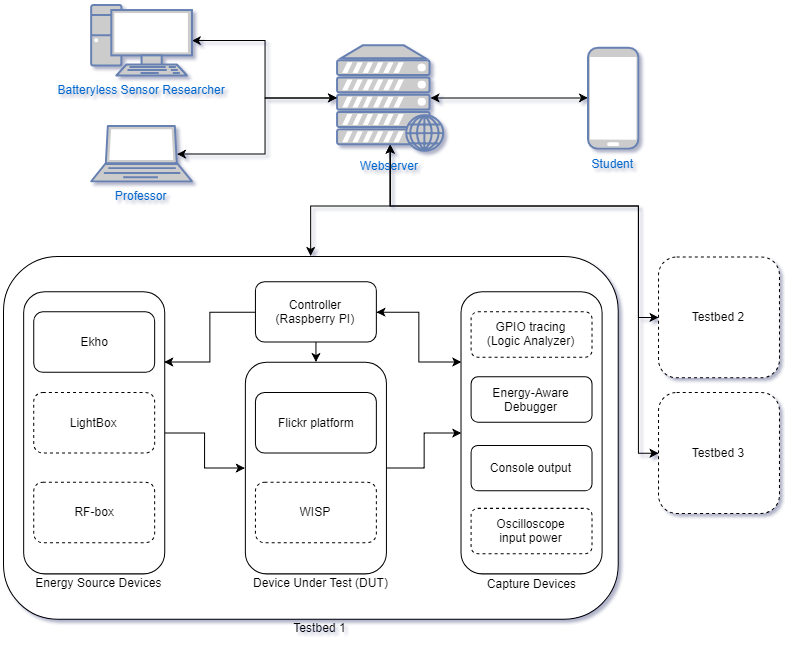
\includegraphics[width=\linewidth]{TestbedArchitecture_v2}
	\caption{Testbed architecture}
	\label{fig:architecture}
\end{figure}


% Bibliography
\bibliographystyle{unsrt}
\bibliography{references}

\end{document}
